\documentclass[scheme=plain,UTF8]{ctexart}
%\documentclass[]{article}
%\usepackage{xeCJK}
\usepackage{needspace}
%\usepackage[nocap]{ctexcap}
\usepackage{enumitem}
\usepackage{color}
\usepackage{longtable}
%\usepackage{longtable,booktabs}
\usepackage{tikz,mathpazo}
\usepackage{tabu}
\usepackage{graphicx}
\usepackage{media9}
\usetikzlibrary{shapes.geometric, arrows}
\usetikzlibrary{calc}
\usepackage[top=2cm,bottom=2cm]{geometry}
\setCJKmainfont[AutoFakeBold]{FangSong_GB2312}
%\setCJKmainfont{FangSong}

%\newcounter{zwbh}
%\begin{list}{\heiti 步骤 \chinese{zwbh}、}
%{\usecounter{zwbh}
% \itemsep=-2pt\labelsep=0.2em}
% \item 建立适当的直角坐标
% \item 找出动点
% \end{list}
\newcounter{mylist}
% 列表环境定义
\newenvironment{myitemize}{%
  \begin{list}{\hspace{2em}\themylist 、}{%
      \usecounter{mylist}%
      \setlength{\topsep}{0pt}%
      \setlength{\partopsep}{0pt}%
      \setlength{\parsep}{0pt}%
      \setlength{\itemsep}{0pt}%
      \setlength{\leftmargin}{0pt}%
      \setlength{\rightmargin}{0pt}%
      \setlength{\labelsep}{0pt}%
      \setlength{\itemindent}{2.0em}%
    }
  } {\end{list} }

% 自定义列表
\newenvironment{Mylist}[4][\chinese{mylist}、]{%
\begin{list}{#1}{\usecounter{mylist}\topsep=0pt\itemsep=0pt\parsep=0pt\partopsep=0pt%
\itemindent=#2\leftmargin=#3\rightmargin=#4}}{\end{list}}
% 二级标题
\newenvironment{sectitle}[1][(\chinese{mylist})、]{%
\begin{list}{#1}{\usecounter{mylist}\topsep=0pt\itemsep=0pt\parsep=0pt\partopsep=0pt%
\itemindent=2em\leftmargin=8mm\rightmargin=0mm}}{\end{list}}
%三级标题
\newcounter{thirdlist}
\newenvironment{thirdtitle}[1][\thethirdlist.]{%
\begin{list}{#1}{\usecounter{thirdlist}\topsep=0pt\itemsep=0pt\parsep=0pt\partopsep=0pt%
\itemindent=2em\leftmargin=8mm\rightmargin=0mm}}{\end{list}}


% 流程图定义基本形状
\tikzstyle{startstop} = [rectangle, rounded corners, minimum width = 2cm, minimum height=1cm,text centered, draw = black, fill = red!40]
\tikzstyle{pros} = [rectangle, rounded corners, minimum width = 2cm, minimum height=1cm,text centered, draw = black, fill = blue!40]
\tikzstyle{io} = [trapezium, trapezium left angle=70, trapezium right angle=110, minimum width=2cm, minimum height=1cm, text centered, draw=black, fill = blue!40]
\tikzstyle{process} = [rectangle, minimum width=3cm, minimum height=1cm, text centered, draw=black, fill = yellow!50]
\tikzstyle{decision} = [diamond, aspect = 3, text centered, draw=black, fill = green!30]
% 箭头形式
\tikzstyle{arrow} = [->,>=stealth]



%\title{\heiti{费用报销制度}}
%\date{}

% \AddEnumerateCounter{\chinese}{\chinese}{}


%\pagestyle{plain}
%%%%%%%%%% ctexcap %%%%%%%%
% \CTEXsetup[name={第,节}, number={\chinese{\section}}]{section}

%%%%%%%%%%%%%%%%%%%
\ctexset {
autoindent=true,
figurename=图,
tablename=表,
appendixname=附录,
% part/pagestyle = empty,
% chapter = {
% format = \raggedright,
% pagestyle = empty,
% },
section = {
name = {,、},
% nameformat= \Large\bf,
aftername = \medskip,
number = \chinese{section},
%number = \arabic{section},
format = \zihao{3},
%break = \Needspace{.5\textheight},
},
subsection = {
name = {(,)},
% nameformat= \Large\bf,
aftername = \medskip,
number = \chinese{subsection},
%number = \arabic{section},
format = \zihao{3},
},
% subsubsection = {
% name = {,.},
% % nameformat= \Large\bf,
% aftername = \space,
% number = \arabic{subsubsection},
% %number = \arabic{section},
% format = \zihao{3},
% nameformat = \bigskip\hfill,
% %beforeskip = 12pt,
% },
% paragraph = {
% name = {,.},
% % nameformat= \Large\bf,
% aftername = \space,
% %number = \arabic{subsubsection},
% %number = \arabic{section},
% format = \zihao{3},
% nameformat = \bigskip\hfill,
% %beforeskip = 12pt,
% }
}

\begin{document}
%\maketitle
%\thispagestyle{empty}
\zihao{3}
\begin{center}
\textbf{费用报销制度}
\end{center}
\vspace{3ex}
%\zihao=-3
\section{目的}
为规范公司的费用报销流程,加强对费用报销的监管,特制订本制度。

\section{适用范围}
本制度适用于深圳市巴达木科技有限公司及其关联公司。

\section{报销中的原则责任}

\begin{sectitle}
  \item 原则
		\begin{thirdtitle}
			\item 预算管理原则:在公司预算范围内进行费用报销。无预算或超出预算的费用,须先申请增补预算再报销。
			\item 客观性原则:基于公司实际业务和公司费用标准,合理发生费用,不弄虚作假。
			\item 合法性原则:严格遵守国家和公司的有关规定,取得发票或税务认可的票据。
			\item 及时性原则:在要求时限内完成费用报销,不超时、不跨期;当月的费用必须在次月内报销。
		\end{thirdtitle}
  \item 责任
		\begin{thirdtitle}
			\item 报销人:必须如实填报各项报支凭证和申请上规定的项目,并对所报销的业务真实性承担责任。
			\item 部门负责人:审核部门人员的报销费用是否真实、是否合理、是否合规;
			\item 财务部:对报销的凭证的真实性、合法性、合规性进行审核,对不合规定的报销凭证予以退回,
			\item 对符合规定的凭证进行批准。审核报销单据是否符合费用报销理制度要求、审核报销发票是否符合税务要求、
			\item 复核报销单据是否计算正确、复核借款是否冲销、复核审批手续是否完整。对报销凭证的完整性、有效性及审批流程的正确性承担责任。
		\end{thirdtitle}
\end{sectitle}

\section{费用报销时间}

\begin{sectitle}
	\item 费用报销人当月25日前发生的费用在当月提交到财务,25日以后发生的费用可以在次月提交,逾期未提交不予报销。
	\item 离职员工办理离职手续前,须完成个人费用的报销,离职后不允许他人代报销。
	\item 财务人员每周五或周六付款一次。
\end{sectitle}


\section{报销流程}

报销人须跟进审批流程,报销人填写报销单并贴好单据后,当部门负责人审核完成进入财务会计审核环节,
财务部审核无误后交总经理审批,审批完成后由出纳付款。
% https://www.cnblogs.com/fly2mato/p/7994200.html
\begin{figure}[htbp]
\centering
\begin{tikzpicture}[node distance=2cm]
%定义流程图具体形状
\node (start) [startstop] {填写报销单};
% \node (pro1) [startstop, right of=start] {p1};
\node (pro1) [pros, right of=start,  xshift=1.5cm] {部门负责人审核};
\node (pro2) [startstop, right of=pro1,  xshift=1.5cm] {财务审核};
\node (pro3) [pros, right of=pro2,  xshift=1cm] {总经理审核};
\node (pro4) [startstop, right of=pro3,  xshift=1cm] {出纳付款};
% \node (pro1) [process, below of=start, yshift=-0.2cm, left of=start, xshift=-1cm] {PROCESS 1};
% \node (pro2) [process, right of=pro1, xshift= 4cm] {PROCESS 2};
% \node (in1) [io, below of=pro1, yshift= -0.2cm, right of=pro1, xshift=1cm] {IO};
% \node (pro3) [process, below of=in1, yshift= -0.2cm] {PROCESS 3};
% \node (pro4) [process, below of=pro3, yshift= -0.2cm] {PROCESS 4};
% \node (in2) [io, below of=pro4, yshift= -0.2cm] {IO 2};
% \node (dec1) [decision, below of=in2, yshift= -0.2cm] {DECISION};
%\node (stop) [startstop, below of=dec1] {end};

%连接具体形状
\draw [arrow](start) -- (pro1);
\draw [arrow](pro1) -- (pro2);
\draw [arrow](pro2) -- (pro3);
\draw [arrow](pro3) -- (pro4);
% \draw [arrow](in1) -- (pro3);
% \draw [arrow](pro3) -- (pro4);
% \draw [arrow](pro4) -- (in2);
% \draw [arrow](in2) -- (dec1);
% \draw [arrow](dec1) -- ($(dec1.east) + (1.5,0)$) node[anchor=north] {NO} |- (pro3);
% \draw [arrow](dec1) -- node[anchor=west] {YES} (stop);
\end{tikzpicture}
\caption{\label{fig: } 审批流程图}
\end{figure}
\nopagebreak

\section{费用报销单要求}

\begin{Mylist}[(\chinese{mylist})、]{2em}{8mm}{0mm}
	\item 各类费用应按实际发生的业务内容实事求是、准确无误填写费用
	报销单。手工填写的费用报销单一律不允许涂改,如有修改一律无效。一
	张费用报销单只能对一个公司的费用进行申请报销。不能多张报销单贴在
	一起。
	\item 费用报销的摘要描述应能清楚描述业务的基本内容,对不能描述
	清楚业务内容的,应同时提供相关的说明文件。
	\item 所有报销事项,应有相关凭据,能证明事项真实发生。
	\item 有发票的和没有发票的单据应分开报销,不能贴在同一张报销单上,发票抬头必须是公司名称,不能为个人。
\end{Mylist}

\section{发票要求}
%       \item公司开票资料}
% 1)	公司名称:\textcolor{red}{深圳巴达木科技有限公司}\\\indent
% 2)	税务编码:\textcolor{red}{9144030006499864XA}\\\indent
% 3)	地址及电话:\textcolor{red}{深圳市宝安区新安街道28区大宝路49-1号金富来商务大厦一楼111室0755-85285522}\\\indent
% 4)	开户行及账号:\textcolor{red}{中国工商银行股份有限公司深圳宝民支行4000092509100249944}\\\indent
% 增值税专用发票,需包含以上四项内容;增值税普通发票,至少应包含公司名称及税务编码。
\begin{sectitle}
	\item 报销的发票、收据类型
		\begin{thirdtitle}
			\item 增值税专用发票;
			\item 增值税普通发票(含增值税电子普通发票);
			\item 通用机打发票;
			\item 通用定额发票;
			\item 客运发票、轮船票、出租车发票、火车票、飞机票行程单、以及通行费发票;
			\item 行政事业单位提供的财政监制收据;
			\item 其他税务认可的票据;
			\item 用餐费用必须有发票;
			\item 叫车送货的费用:达达、快狗、货拉拉、滴滴必须提供发票;
			\item 天猫购物可以开发票的商品必须提供发票。
		\end{thirdtitle}
	费用报销须提供以上发票或票据,其他凭据均视为不能提供发票。
	\item 发票内容,须与实际业务一致。与实际业务不相符的发票,财务部应予以退回。
	\item 增值税电子普通发票,报销人需自行打印。
	%      \item发票丢失的费用原则上不允许报销,经部门负责人、总经理批准的,可使用替票报销实际业务金额的\textcolor{red}{85\%}。}
\end{sectitle}

\section{明细费用管理要求}
\begin{sectitle}
   \item 外出费用
		\begin{thirdtitle}
			\item 市内外勤人员,交通费用实报实销。
			\item 原则上选择公交、地铁,特殊原因需经部门负责人批准后可报销。允许报销费用的情况如下:
			因公用车发生的费用,如加油费、过路费等可申请报销,但在公务过程中发生的违章以及其他事故不予报销。因私事发生的车辆费用也不予报销。
			员工外出办公,携带大件物品不便于乘坐公共交通的。
			其他经部门负责人批准的特殊情况。
			交通费报销,包括乘坐交通工具的费用;对于交通费应当提前在钉钉报备,费用报销须按业务事项内容逐笔如实填写乘车日期、起止地点、办事内容、金额,需备注乘车原因,按照附件一《市内交通费明细》格式作为附件上传钉钉。
			报销要求:能开票的平台需提供发票报销,如滴滴、达达等。不能开发票的平台,应提供行程单。
		\end{thirdtitle}
%       \item 差旅费

% 1)	差旅费报销范围:出差人异地出差,公司至出差地交通费、出差地市内交通费、出差地住宿费用、出差期间补助。\\\indent
% 2)	员工异地出差,需先在钉钉填写出差申请单,详细预计出差的目的地、出差事项、出差时间等信息,由部门负责人签批。\\\indent
% 3)	在钉钉提交差旅费报销单,须关联对应的出差申请单,无出差申请单的差旅费不予报销。\\\indent
% 4)	公司至出差地交通费交通工具选择:\\\indent
% A.	大于1000公里,可选择乘坐飞机(经济舱)、高铁(二等座)、火车(硬座,如乘坐时间超过4小时可选择硬卧);\\\indent
% B.	小于等于1000公里,可选择乘坐高铁(二等座)、火车(硬座,如乘坐时间超过4小时可选择硬卧)、汽车、轮船;如乘坐飞机整体费用(含机票、机场建设、燃油附加)低于其他交通工具,可选择乘坐飞机。\\\indent
% 5)	出差住宿费\\\indent
% A.	出差酒店住宿,原则上选择经济型连锁酒店,如7天、如家等。\\\indent
% B.	住宿费标准:\\\indent
% a)	一线城市(北京、上海、广州、深圳):300元/晚;\\\indent
% b)	二线城市(除一线城市以外的省会城市、厦门、苏州、青岛、大连):250元/晚;\\\indent
% c)	三线及以下城市(除一线、二线以外的城市):200元/晚。\\\indent
% C.	同性别两位同事一同出差,报销一个标准房间的费用。 \\\indent
% 6)	两位(含两人位)同事以上共同产生费用并只开具一张发票,由一人报销,其他同事须在发票背面签名确认。\\\indent
% 7)	出差补助50元/天,无需提供发票。如出差期间产生业务招待费,则当天的出差补助不能报销。\\\indent


   \item 业务费
		\begin{thirdtitle}
		  \item 范围:因公发生的对外业务招待费用。
		  \item 事项:业务费须事先在钉钉上提交《业务费申请单》,填写招待事由、招待对象,以及预计花费,经总经理审批同意后再使用;
		  \item 报销:业务招待费应当在钉钉填写费用报销单-业务招待费用。因故未能提前申请的,应事后补单。否则,不予报销。
				所有业务费用报销时需在费用报销单注明业务费用发生的招待事由、招待对象(指被请人员的所属公司、部门、职级或姓名)。
		\end{thirdtitle}
%       \item车辆使用费}

% 1)	范围:公司员工前往临近城市出差,由于交通原因,选择公车私用所产生的车辆使用费用。\\\indent
% 2)	事项:因公用车发生的费用,如加油费、过路费等可申请报销,但在公务过程中发生的违章以及其他事故不予报销。因私事发生的车辆费用也不予报销。
% \textcolor{red}{公司原则上不建议私车公用。如确有需要,用车人须向部门负责人报备。}\\\indent
% 3)	用车人在钉钉上提交报销单,须注明用车起止地点、用车日期,以及单程距离。\\\indent
% 4)	按照往返路程距离1元/公里报销,报销人提供加油票、停车票、过路费均可。

%       \item\textcolor{red}{部门团队建设费及生日会}}
%       \item团队建设费}

% A.	公司一级部门以每人(待定)元/月度为标准提供团建经费,由部门负责人组织活动,季度内在预算标准内实报实销。\\\indent
% B.	团队建设费报销时需与其费用分开填写并注明部门活动内容,如:聚餐、K歌等。须在报销单上列明或者上传参加人员名单。\\\indent
% (属于跨团队的原则上在场级别最高领导买单,后期不再同意。)\\\indent
% C.	团队建设费报销时须提供活动相对应发票,如餐饮费、交通费、场地费等。

   \item 办公用品、固定资产、工具等其他零星采购
		\begin{thirdtitle}
		  \item 办公用品必须先在前台钉钉上提采购申请,然后由前台统一采购,其他人不得自行采购。
		  \item 固定资产、工具、劳务服务等零星采购由请购人在钉钉上提交申请,未经审批不得报销。

		  \item 其他杂项费用

		  \item 范围:以上费用以外的开支。
		  \item 本着开源节流、合理必须的原则,其他杂费和正常办公费用按公司审批权限审批报销。
		\end{thirdtitle}
\end{sectitle}

\section{各项费用报销清单}

% Table generated by Excel2LaTeX from sheet 'Sheet1'
\begin{longtable}{|c|p{30mm}|p{40mm}|p{50mm}|}
%  \centering
  % \caption{Add caption}
%    \begin{tabular}{|p{4.19em}|p{4.19em}|p{4.19em}|>{\centering}p{4.19em}|}
    \hline
    \textbf{报销单类型} & \textbf{费用申请单} & \textbf{纸质报销资料} & \textbf{电子报销资料(附件上传或在报销单上注明)} \\
    \hline
    市内交通费 & 无     & 交通发票  & 交通费用明细 \\
    \hline
    差旅费   & 出差申请单 & 报销单、机票/火车票/汽车票、住宿发票、交通发票 & 出差事由、出差地点及出差日期 \\
    \hline
    业务招待费  & 业务费申请单 & 业务费用发票 & 招待事由、招待对象 \\
    \hline
    % 市场推广费 & 无     & 发票、采购明细(如发票包含采购明细则不需要提供)、签收表及签收人员身份证复印件(外请临时人员) & 推广方案、费用明细 \\
    % \hline
    通讯费   & 无     & 个人通讯费发票 & \multicolumn{1}{c|}{} \\
    \hline
    办公费用  & 无     & 发票    & 费用明细 \\
    % \hline
    % 会议费   & 无     & 发票    & 费用明细 \\
    % \hline
    % 员工福利费 & 无     & 发票    & 费用明细、人员名单 \\
    % \hline
    % 团队建设费 & 无     & 餐饮发票、交通发票、 & 费用明细、人员名单 \\
    \hline
    车辆使用费 & 无     & 加油票、停车票、过路费发票 & 用车事由、起止地点 \\
    \hline
    快递费   & 无     & 快递费发票、快递单存根联 & 快递明细 \\
    \hline
    其他费用开支 & 无     & 发票、其他业务资料 & 费用明细 \\
    \hline
 %   \end{tabular}%
  % \label{tab:addlabel}%
\end{longtable}%

%报销一律用中文名

\section{单据填写}
\begin{sectitle}                                                                                                                                                                                                                                                                                                                                         
      \item 所有费用报销在钉钉填写并提交报销单,差旅费提交《差旅费报销单》,业务费提交《业务费报销单》,其他费用提交《费用报销单》。
      \item 票据粘贴完毕后,必须在粘贴底单上用黑色签字笔写上钉钉审批编码,以及报销人姓名(\textcolor{red}{报销一律用中文名})。
      \item 使用替票的费用报销,须按照代替发票的票面内容填写报销信息,在钉钉报销说明中注明替代事由及原费用情况。(替票处理)
\end{sectitle}

\section{单据粘贴}
\begin{sectitle}
      \item \textcolor{red}{在底单写上钉钉编码及报销人姓名,每一个钉钉审批编码,对应粘贴一份原始单据。不得多个钉钉审批编码单据粘贴为一份原始单据。}
      \item 必须将原始单据粘贴在粘贴底单上、必须使用胶水粘贴整齐,不得使用订书机。 
      \item 票据粘贴以左边和上边对整齐,按发票面积大小分类,面积小的单据贴下面,面积大的单据贴上面,并依次粘贴。
      \item 所有报销单据粘贴要求整齐、美观。(黏贴操作详见附录)\\[1ex]
	 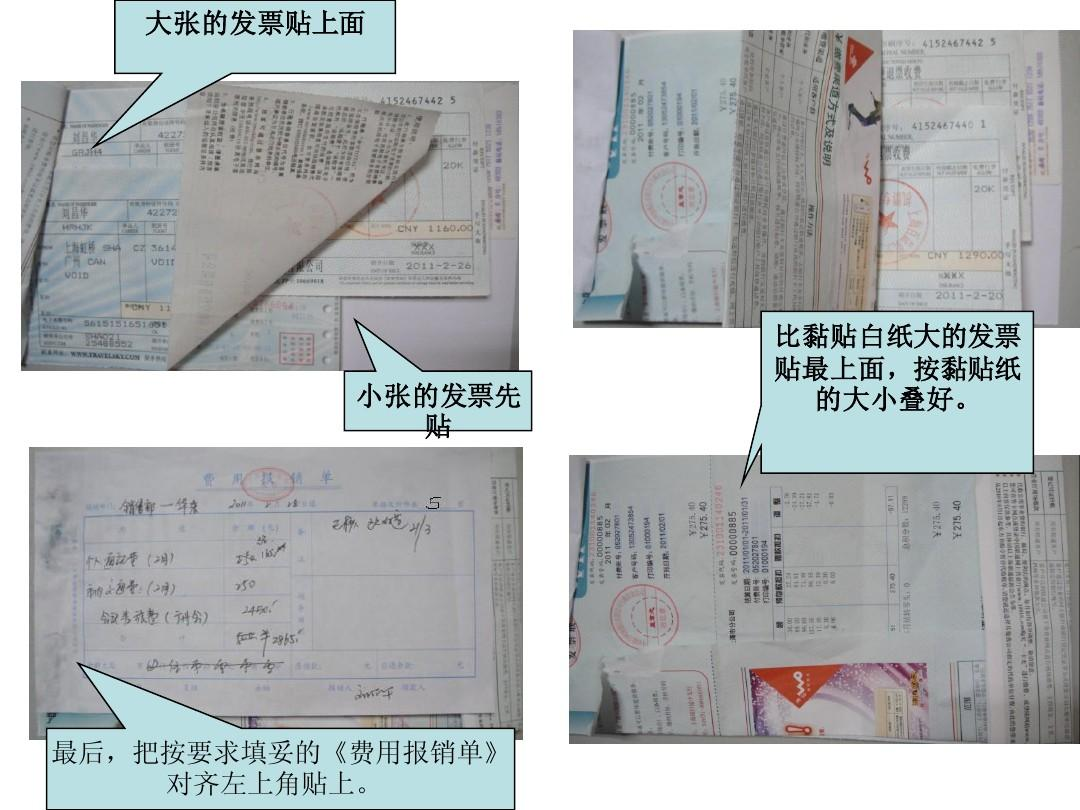
\includegraphics[height=0.5\linewidth,width=0.5\linewidth]{fapiaoniantie5}\hspace{2em}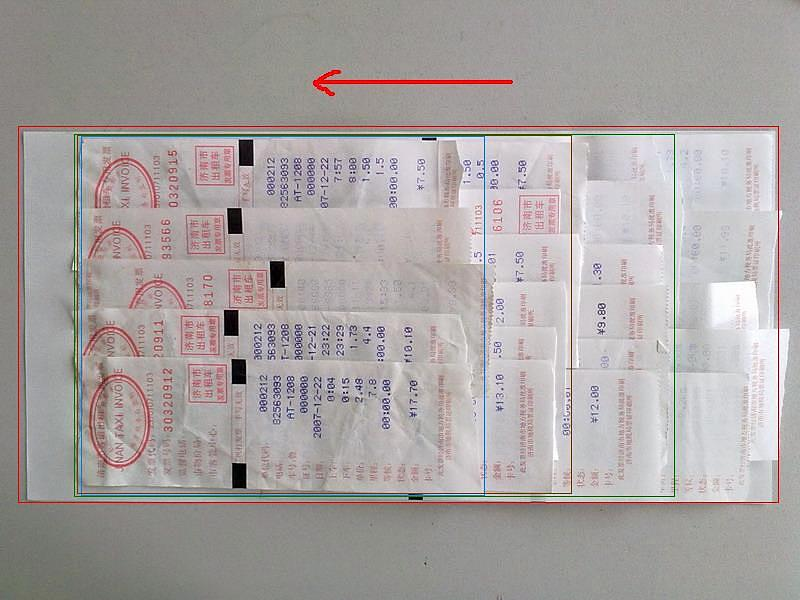
\includegraphics[height=0.45\linewidth,width=0.45\linewidth]{fapiaoniantie}
\end{sectitle}

\newpage
\appendix
\section{附录}
\vspace{2ex}
为了确保视频能够播放,请用Acrobat Reader 打开观看pdf :-)
\begin{Mylist}[示例\themylist.]{2em}{8mm}{0mm}
% using https://ksv-video-publish.cdn.bcebos.com/62886b8d0091c000894cc32ae667258b39743f59.mp4?auth_key=1624607099-0-0-d8ca26f319a8db0e4ab0ed0f8d1f06bd
\item \hfill\\[1ex]
\includemedia[width=0.5\linewidth,height=0.28\linewidth,activate=pageopen,
passcontext,
transparent,
addresource=fapiaoniantiev1.mp4,
flashvars={source=fapiaoniantiev1.mp4}
]{
\includegraphics[height=0.28\linewidth,width=0.5\linewidth]{fapiaoniantiev1}}{VPlayer.swf}
	%\item 
	% using a .mp4; downloaded from https://ksv-video-publish.cdn.bcebos.com/d8e830578120df57145a518d393627c7020dce22.mp4?auth_key=1624607099-0-0-687aa056b7e135a16125aa48ad6e4e97
\item \hfill\\[1ex]
\includemedia[width=0.5\linewidth,height=0.28\linewidth,activate=pageopen,
passcontext,
transparent,
addresource=fapiaoniantiev.mp4,
flashvars={source=fapiaoniantiev.mp4}
]{
\includegraphics[height=0.28\linewidth,width=0.5\linewidth]{fapiaoniantiev}}{VPlayer.swf}
\end{Mylist}


\end{document}